\documentclass[aspectratio=169,xcolor=dvipsnames]{beamer}
\usetheme{SimpleDarkBlue}

\usepackage{hyperref}
\usepackage{graphicx}
\usepackage{booktabs}
\usepackage{amssymb}
\usepackage{amsmath}
\usepackage{tikz}
\usepackage{xcolor}
\usepackage{caption}
\usepackage{amsthm}

\title{Sublinear Algorithms for $(\Delta+1)$ Vertex Coloring}

\author{
	Mohammad Hosein Rabiee
	\and
	Amir Hosein Karimzadegan \\
	\and
	Mohammad Reza Ahmadi
	\and
	Behrad Sanei
}

\institute
{
	Department of Computer Science and Statistics \\
	Faculty of Mathematics \\
	K. N. Toosi University of Technology
}
\date{}

\begin{document}
	
	\begin{frame}
		\titlepage
	\end{frame}
	
	\begin{frame}{Overview}
		\tableofcontents
	\end{frame}
	
	\section{Graph Coloring}
	
	\begin{frame}{Graph Coloring}
		
		\begin{itemize}
			\item Assign a small number of colors to vertices of a graph \textcolor{blue}{$G(V,E)$} such that there \alert{no monochromatic edges} (has the same color on both endpoints).
			\item A \textcolor{blue}{proper \alert{$c$}-coloring} of a graph \textcolor{blue}{$G(V,E)$}:
			\begin{itemize}
				\item assigns a color from the palette $\{1, 2, \ldots, c\}$ to all vertices $V$ of $G$,
				\item no \alert{monochromatic edges}
			\end{itemize}
		\end{itemize}
		
		\begin{figure}[h]
			\centering
			\begin{minipage}[b]{0.45\textwidth}
				\centering
				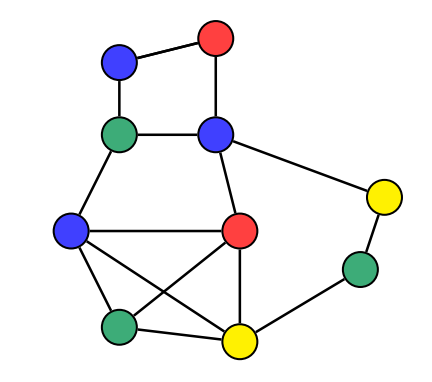
\includegraphics[width=0.5\textwidth]{images/4GraphColoring.png}
				\caption*{a proper \alert{4}-coloring of \alert{$G$}}
			\end{minipage}
			\hfill
			\begin{minipage}[b]{0.45\textwidth}
				\centering
				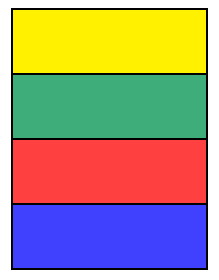
\includegraphics[width=0.3\textwidth]{images/ColorsPalette.png}
				\caption*{a palette of \alert{$4$} colors}
			\end{minipage}
		\end{figure}
		
	\end{frame}
	
	\begin{frame}{Graph Coloring}
		
		\begin{itemize}
			\item A central problem in graph theory and computer science.
			\item But the task of coloring a graph with a \alert{minimum number of colors} is a notoriously hard problem.
		\end{itemize}
		\begin{block}{Theorem [Feige and Killian '98, Zuckerman '07]}
			For any \alert{$\epsilon>0$}, it is NP-hard to approximate the number of colors needed to within a factor \alert{$n^{1-\epsilon}$}.
		\end{block}
		\footnotesize
		\nocite{*}
		\bibliographystyle{apalike}
		\bibliography{FeigeKilian98-Zuckerman07.bib}
		
	\end{frame}
	
	\begin{frame}{Graph Coloring}
		\begin{itemize}
			\item So in many applications, we instead focus on coloring a graph using a number of colors based on some \textcolor{blue}{graph parameter}.
			\item An important and well-studied case: \alert{$(\Delta + 1)$} coloring
			\begin{itemize}
				\item \alert{$\Delta$} : maximum degree
			\end{itemize}
		\end{itemize}
		\begin{block}{}
			Every graph admits a \alert{$(\Delta+1)$} coloring
		\end{block}
		\begin{itemize}
			\item Iterate over the vertices in an arbitrary order
			\item Assign each vertex a color that is not in its neighborhood
			\item Since the max-degree is \alert{$\Delta$}, such a color always exists
		\end{itemize}
		The runtime of this algorithm is \alert{$O(m+n)$} time which is clearly optimal as we need this much time simply to read the input.
	\end{frame}
	
	\section{Sublinear Algorithms}
	
	\begin{frame}{Sublinear Algorithms}
		\begin{itemize}
			\item How about \textcolor{blue}{massive graphs}? Is there an even more efficient algorithm?
		\end{itemize}
		
		\begin{alertblock}{}
			Can we design \textcolor{blue}{sublinear algorithms} for \alert{$(\Delta + 1)$}-coloring problem in modern models
			of computation for processing massive graphs?
		\end{alertblock}
		
		\begin{itemize}
			\item This paper answer this fundamental question in the affirmative for modern models of computation.
		\end{itemize}
		
	\end{frame}
	
	\begin{frame}{Sublinear Algorithms}
		\begin{itemize}
			\item Sublinear means sublinear in the number of \textcolor{blue}{edges}. Since the output of \alert{$(\Delta + 1)$}-coloring is always \textcolor{blue}{linear} in the number of \textcolor{blue}{vertices}.
		\end{itemize}
		
		\begin{alertblock}{}
			Can compute a \alert{$(\Delta + 1)$}-coloring by examining only a \textcolor{blue}{tiny fraction} of the edges in a graph?
		\end{alertblock}
		\begin{itemize}
			\item Based on the computational models, we may want \textcolor{blue}{sublinear time}, \textcolor{blue}{space}, or \textcolor{blue}{communication} algorithms.
		\end{itemize}
		
	\end{frame}
	
	\begin{frame}{Sublinear Algorithms}
		
		\begin{enumerate}
			\item \textcolor{blue}{Sublinear time} algorithms:
			\begin{itemize}
				\item Process the graph \textcolor{blue}{faster} than even reading the entire input.
			\end{itemize}
			
			\vspace{2.5em}
			
			\item \textcolor{blue}{Streaming} algorithms:
			\begin{itemize}
				\item Process the graph \textcolor{blue}{on the fly} with \textcolor{blue}{limited memory}.
			\end{itemize}
			
			\vspace{2.5em}
			
			\item \textcolor{blue}{Massively parallel computation (MPC)} algorithms:
			\begin{itemize}
				\item Process the graph in a \textcolor{blue}{distributed} fashion with \textcolor{blue}{limited communication}.
			\end{itemize}
		\end{enumerate}
		
	\end{frame}
	
	\section{Main Results}
	
	\begin{frame}{Main Results}
		Surprisingly, we can get highly efficient sublinear algorithms for
		\alert{(\(\Delta + 1\))}-coloring in
		\textcolor{blue}{three models of computation}.
		
		\vspace{1em}
		All algorithms are \textcolor{blue}{randomized} and behave as follows:
		\begin{itemize}
			\item either output a valid \alert{(\(\Delta + 1\))}-coloring (w.h.p.), or
			\item output FAIL.
		\end{itemize}
		
		\vspace{1em}
		these algorithms \textcolor{blue}{\textbf{never output}} an invalid coloring.
	\end{frame}
	
	\begin{frame}{Result 1: Sublinear Time Algorithms}
		
		The standard query model for dense graphs:
		\begin{itemize}
			\item Degree queries: what is the degree of the vertex \textcolor{red}{$v$}?
			\item Pair queries: is \textcolor{red}{$(u, v)$} an edge?
			\item Neighbor queries: what is the \textcolor{red}{$k$}-th neighbor of the vertex \textcolor{red}{$v$}?
		\end{itemize}
		
		\vspace{1em}
		\textcolor{blue}{\textbf{Prior Results:}} \\
		No sublinear time algorithm for \textcolor{red}{$(\Delta + 1)$} coloring. \\
		Fastest algorithm: the \textcolor{red}{$O(n^2)$} time greedy algorithm.
		
	\end{frame}
	
	\begin{frame}{Result 1: Sublinear Time Algorithms}
		
		The standard query model for dense graphs:
		\begin{itemize}
			\item Degree queries: what is degree of the vertex {\color{red}$v$}?
			\item Pair queries: is {\color{red}$(u,v)$} an edge?
			\item Neighbor queries: what is the {\color{red}$k$}-th neighbor of the vertex {\color{red}$v$}?
		\end{itemize}
		
		\vspace{0.5em}
		\textcolor{blue}{\textbf{Paper's Result:}}
		
		\vspace{0.5em}
		\begin{block}{}
			\centering
			An \textcolor{red}{$\tilde{O}(n\sqrt{n})$} time algorithm for \textcolor{red}{$(\Delta + 1)$} coloring.
		\end{block}
		
		\begin{itemize}
			\item Queries are chosen {\color{blue}non-adaptively}(in parallel).
			\item {\color{red}$\Omega(n\sqrt{n})$} query {\color{blue}lower bound} even for adaptive algorithms.
		\end{itemize}
		
	\end{frame}
	
	\begin{frame}{Result 2: Streaming Algorithms}
		
		\textcolor{blue}{Semi-streaming} algorithms:
		\begin{itemize}
			\item Edges are appearing one by one in a stream.
			\item Process the stream in one pass and \textcolor{red}{$\tilde{O}(n)$} space.
		\end{itemize}
		
		\vspace{0.5em}
		\textcolor{blue}{Prior Results:}
		\begin{itemize}
			\item No single-pass streaming algorithm for {\color{red}$(\Delta + 1)$} coloring with {\color{red}$o(n^2)$} space even in insertion-only streams.
			\item \underline{Parallel to this work.} \textcolor{blue}{Easier} problem of {\color{red}$(\Delta + o(\Delta))$}: a semi-streaming algorithm using sulinear space by {\color{green!50!black}[Bera and Ghosh, 2018]}.
		\end{itemize}
		
	\end{frame}
	
	\begin{frame}
		\frametitle{Result 2: Streaming Algorithms}
		
		\textcolor{blue}{Semi-streaming} algorithms:
		\begin{itemize}
			\item Edges are appearing one by one in a stream.
			\item Process the stream in one pass and \textcolor{red}{$\tilde{O}(n)$} space.
		\end{itemize}
		
		\vspace{0.5em}
		\textcolor{blue}{Paper's Result:}
		
		\begin{block}{}
			\centering
			A single-pass \textcolor{red}{$\tilde{O}(n)$} space streaming algorithm for {\color{red}$(\Delta + 1)$} coloring.
		\end{block}
		
		\begin{itemize}
			\item {\color{red}$\Omega(n)$} space is clearly \textcolor{blue}{necessary} for this problem(optimal).
			\item This algorithm works even in \textcolor{blue}{dynamic graph streams}.
		\end{itemize}
		
	\end{frame}
	
	\begin{frame}{Result 3: MPC Algorithms}
		
		MPC algorithms with \textcolor{blue}{{$\tilde{O}(n)$}} memory per-machine:
		\begin{itemize}
			\item Edges are partitioned arbitrarily across multiple machines.
			\item Machines can send and receive \textcolor{red}{$\tilde{O}(n)$} messages in synchronous rounds.
		\end{itemize}
		
		\vspace{0.5em}
		\textcolor{blue}{Prior Results:}
		\begin{itemize}
			\item An \textcolor{red}{$\mathcal{O}(\log \log \Delta \cdot \log^* (n))$} round algorithm with \textcolor{red}{$\tilde{O}(n)$} memory per-machine for \textcolor{red}{$(\Delta + 1)$} coloring \textcolor{green!50!black}{[Parter, 2018]}.
			
			\item \underline{Parallel to this work.} The round-complexity improved to \textcolor{red}{$\mathcal{O}(\log^* (n))$} rounds \textcolor{green!50!black}{[Parter and Su, 2018]}.
			
			\item \textcolor{blue}{Easier} problem of \textcolor{red}{$(\Delta + o(\Delta))$} coloring: an \textcolor{red}{$\mathcal{O}(1)$} round algorithm with \textcolor{red}{$n^{1+\Omega(1)}$} memory \textcolor{green!50!black}{[Harvey et al., 2018]}.
		\end{itemize}
		
	\end{frame}
	
	\begin{frame}{Result 3: MPC Algorithms}
		
		MPC algorithms with \textcolor{blue}{{$\tilde{O}(n)$}} memory per-machine:
		\begin{itemize}
			\item Edges are partitioned arbitrarily across multiple machines.
			\item Machines can send and receive \textcolor{red}{$\tilde{O}(n)$} messages in synchronous rounds.
		\end{itemize}
		
		\vspace{1em}
		\textcolor{blue}{Paper's Result:}
		\begin{block}{}
			An \textcolor{red}{$\mathcal{O}(1)$} round \textcolor{red}{$\tilde{O}(n)$} memory MPC algorithm for \textcolor{red}{$(\Delta + 1)$} coloring.
		\end{block}
		
		\begin{itemize}
			\item This algorithm only requires \textcolor{blue}{one round} assuming \textcolor{blue}{public randomness}(optimal).
			\item The first \textcolor{blue}{constant round} MPC algorithm with \textcolor{red}{$\tilde{O}(n)$} memory for one of ``classic four local distributed graph problems".
		\end{itemize}
		
	\end{frame}
	
	\section{Palette Sparsification Theorem}
	
	\begin{frame}{Palette Sparsification Theorem}
		
		\begin{alertblock}{}
			How do we design these Sublinear Algorithms?
		\end{alertblock}
		\begin{block}{Palette Sparsification Theorem}
			Let \alert{$G(V,E)$} be any \alert{$n$-vertex} graph and \alert{$\Delta$} be
			the maximum degree in \alert{$G$}. Suppose for each vertex \alert{$v \in V$} , we \textcolor{blue}{independently} pick a set \alert{$L(v)$} of colors of size
			\alert{$\Theta(log n)$} \textcolor{blue}{uniformly} at random from \alert{$\{1, \dots, \Delta + 1\}$}. Then \textcolor{blue}{with high probability} there exists a proper coloring \alert{$C : V \mapsto \{1, \dots, \Delta + 1\}$} of \alert{$G$} such that for all vertices \alert{$v \in V$} , \alert{$C(v) \in L(v)$}.
		\end{block}
		
	\end{frame}
	
	\begin{frame}{Palette Sparsification Theorem: Illustration}
		\begin{figure}[h]
			\centering
			\begin{minipage}[b]{0.45\textwidth}
				\centering
				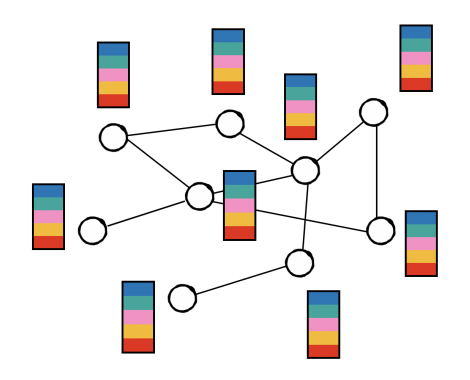
\includegraphics[width=1\textwidth]{images/PaletteSparsification1.png}
				\caption*{(a) A graph \alert{$G = (V, E)$} with its original palettes of \alert{$(\Delta+1)$} colors.}
			\end{minipage}
			\hfill
			\begin{minipage}[b]{0.45\textwidth}
				\centering
				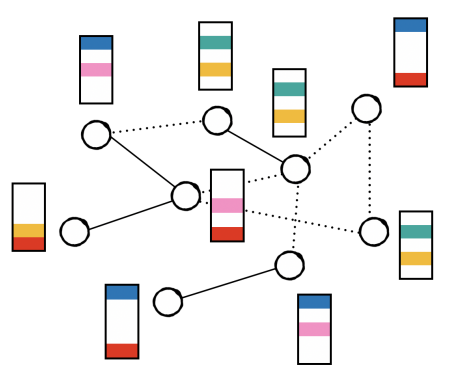
\includegraphics[width=1\textwidth]{images/PaletteSparsification2.png}
				\caption*{(b) The sampled palettes of the vertices and the resulting conflict graph – the dotted edges can be ignored now.}
			\end{minipage}
		\end{figure}
	\end{frame}
	
	\begin{frame}{ColoringAlgorithm}
		\textbf{ColoringAlgorithm$(G,\Delta)$} : A \textcolor{blue}{meta-algorithm} for finding a \alert{$(\Delta+1)$}-coloring in a graph \alert{$G(V,E)$} with
		maximum degree \alert{$\Delta$}.
		\begin{block}{ColoringAlgorithm$(G,\Delta)$}
			
			\begin{enumerate}
				\item Sample \alert{$\Theta(\log{n})$} colors \alert{$L(v)$} \textcolor{blue}{uniformly} at random for each vertex \alert{$v \in V$} (as in \textcolor{blue}{Palette Sparsification Theorem}).
				\item Define, for each color \alert{$c \in \{1, \dots, \Delta + 1\}$}, a set \alert{$\chi_{c} \subseteq V$} where \alert{$v \in \chi_{c} $} iff \alert{$c \in L(v)$}.
				\item Define \alert{$E_{conflict}$} as the set of all edges \alert{$(u, v)$} where both \alert{$u, v \in \chi_{c}$} for some \alert{$c \in \{1, \dots, \Delta + 1\}$}.
				\item \underline{\textcolor{blue}{Construct}} the conflict graph \alert{$G_{conflict}(V,E_{conflict})$}.
				\item \underline{\textcolor{blue}{Find}} a \textcolor{blue}{proper list-coloring} of \alert{$G_{conflict}(V,E_{conflict})$} with \alert{$L(v)$} being the color list of vertex \alert{$v \in V$}.
			\end{enumerate}
		\end{block}
		
	\end{frame}
	
	\begin{frame}{Palette Sparsification Theorem: Properties}
		\begin{block}{Lemma}
			In \textbf{ColoringAlgorithm$(G,\Delta)$}, \textit{with
				high probability}, the output is a valid \alert{$(\Delta + 1)$}-coloring of the graph \alert{$G$}.
		\end{block}
		
		\begin{proof}
			\begin{itemize}
				\item By \textcolor{blue}{Palette Sparsification Theorem}, with high probability there does exist a valid list-coloring of \alert{$G_{conflict}$}.
				\item Since \alert{$E_{conflict}$} contains all possible monochromatic edges that arise in any list-coloring of \alert{$G$}, any valid list-coloring of \alert{$G_{conflict}$}, if one exists, is a valid coloring of the input graph \alert{$G$} and vice versa.
				\item So \alert{$(\Delta + 1)$}-coloring of input graph \alert{$G$} reduces to list-coloring of the graph \alert{$G_{conflict}$}.
			\end{itemize}
		\end{proof}
	\end{frame}
	
	\begin{frame}{Palette Sparsification Theorem: Properties}
		\begin{block}{Lemma}
			In \textbf{ColoringAlgorithm$(G,\Delta)$}, \textit{with
				high probability}, the maximum degree in graph \alert{$G_{conflict}$} is \alert{$O({\log^2{n}})$} and
			thus \alert{$G_{conflict}$} has \alert{$O(n{\log^2{n}})$} edges.
		\end{block}
		
		\begin{block}{Proof.}
			\begin{itemize}
				\item Fix any vertex $v \in V$ and its list of colors $L(v)$
				\item Let $K$ be the number of colors sampled by each vertex.
				\item For any neighbor $u$ of $v$ in $G$, let $X_u \in \{0, 1\}$ be an indicator random variable which is $1$ if and only if $v$ is a neighbor of $u$ in $G_{conflict}$
				\item For $u$ to be a neighbor of $v$ in $G_{conflict}$, $L(u) \cap L(v)$ must be non-empty. Thus:
			\end{itemize}
			\[
			\Pr(X_u = 1) = \Pr\left( \bigcup_{c \in L(v)} (c \in L(u)) \right)
			\leq \sum_{c \in L(v)} \Pr(c \in L(u))
			= K \cdot \frac{K}{\Delta + 1}
			= \frac{K^2}{\Delta + 1}
			\]
		\end{block}
	\end{frame}
	
	\begin{frame}
		\begin{alertblock}{Propostion(Chernoff Bound)}
			Suppose $X_1, \dots, X_n$ are independent random variables taking values in $[0, 1]$, and let $X = \sum_{i=1}^{n} X_i$. Then, for any $\epsilon > 0$,
			\[
			\Pr\left( \left| X - \mathbb{E}[X] \right| \geq \epsilon \cdot \mathbb{E}[X] \right) \leq 2 \cdot \exp\left( \frac{-\epsilon^2 \cdot \mathbb{E}[X]}{2 + \epsilon} \right).
			\]
		\end{alertblock}
		
		\begin{block}{Proof(Continued).}
			Moreover, $\deg_{G_{conflict}}(v) = \sum_{u \in N_G(v)} X_u$ and thus:
			
			\[
			\mathbb{E}[\deg_{G_{conflict}}(v)] \leq \Delta \cdot \frac{K^2}{\Delta + 1} = O(\log^2 n),
			\]
			As $\deg_{G_{conflict}}(v)$ is the sum of independent $0$-$1$ random variables $X_u$ for $u \in N_G(v)$, we can apply the Chernoff bound (with $\epsilon = 10$) and obtain:
			\[
			\Pr\left(\deg_{G_{conflict}}(v) \geq 10 \cdot \mathbb{E}[\deg_{G_{conflict}}(v)]\right) \leq 2 \cdot \exp\left( \frac{-100 \log^2 n}{12} \right) < \frac{1}{n^8}.\qed
			\]
		\end{block}
	\end{frame}
	
	\begin{frame}{Palette Sparsification Theorem: Results}
		\begin{itemize}
			\item Construction of \alert{$G_{conflict}$} is \textcolor{blue}{non-adaptive}.
			\item The graph \alert{$G_{conflict}$} is very sparse.
		\end{itemize}
		\begin{alertblock}{}
			\textcolor{blue}{Palette Sparsification Theorem} thus allows \textcolor{blue}{non-adaptive sparsification} of a graph with \alert{$O(n\Delta)$} edges to a graph with \alert{$\tilde{O}(n)$} while preserving \alert{$(\Delta+1)$}-colorability with high probability.
		\end{alertblock}
	\end{frame}
	
	\section{A One-Pass $\tilde{O}(n)$ Space Streaming Algorithm}
	
	\begin{frame}{A One-Pass \textcolor{red}{$\tilde{O}(n)$} Space Streaming Algorithm}
		
		\begin{itemize}
			\item At the start, each vertex \textcolor{red}{$v$} samples \(\Theta(\log n)\) colors independently and uniformly at random -- let \textcolor{red}{$L(v)$} be the set of colors sampled by vertex \textcolor{red}{$v$}.
			
			\vspace{1.5em}
			
			\item When an edge \((u, v)\) arrives in the stream, we now determine its membership in the \textcolor{blue}{conflict graph} by a simple test: if
			$
			\textcolor{red}{L(u)} \cap \textcolor{red}{L(v)} \neq \emptyset,
			$
			add \textcolor{red}{\((u,v)\)} to \textcolor{red}{$E_{\text{conflict}}$}.
			
			\vspace{1.5em}
			
			\item At the end of the stream, we \textcolor{blue}{list-color} the graph
			$
			\textcolor{red}{G_{\text{conflict}}(V, E_{\text{conflict}})}.
			$
		\end{itemize}
		
	\end{frame}
	
	\begin{frame}{{A One-Pass \textcolor{red}{$\tilde{O}(n)$} Space Streaming Algorithm}}
		
		\begin{itemize}
			\item[\scalebox{0.6}{$\blacksquare$}] \textcolor{blue}{Total space} used by algorithm is \textcolor{red}{$\tilde{O}(n)$}:
			\begin{itemize}
				\item space to store the color lists \textcolor{red}{$L(v)$}, which is a total of \textcolor{red}{$\tilde{O}(n)$} space, and
				\item space to store edges in \textcolor{red}{$E_{\text{conflict}}$}, also \textcolor{red}{$\tilde{O}(n)$} space.
			\end{itemize}
			
			\vspace{1em}
			
			\item[\scalebox{0.6}{$\blacksquare$}] We can maintain the set \textcolor{red}{$E_{\text{conflict}}$} in \textcolor{red}{$\tilde{O}(n)$} space even for \textcolor{blue}{dynamic streams} where the graph is revealed by an arbitrary sequence of edge \textcolor{blue}{insertions} and \textcolor{blue}{deletions}.
		\end{itemize}
		
	\end{frame}
	
	\section{Maintaining Algorithm For Dynamic Streams}
	
	\begin{frame}{Maintaining Algorithm For Dynamic Streams}
		
		\begin{block}{Theorem}
			\textit{There exists a randomized single-pass semi-streaming algorithm that given a graph \textcolor{red}{$G$} with maximum degree \textcolor{red}{$\Delta$} presented in a dynamic stream, with high probability finds a \textcolor{red}{$(\Delta + 1)$} coloring of \textcolor{red}{$G$} with using \textcolor{red}{$\tilde{O}(n)$} space and polynomial time.}
		\end{block}
		
	\end{frame}
	
	\begin{frame}{Maintaining Algorithm For Dynamic Streams}
		
		\begin{alertblock}{}
			Proposition: \textit{There exists an streaming algorithm that given a subset \textcolor{blue}{$P \subseteq V\times V $} of pairs of vertices and an integer \textcolor{blue}{$k \geq 1$} at the beginning of a dynamic stream, outputs with high probability a set \textcolor{blue}{$S$} of \textcolor{blue}{$k$} edges from the edges in \textcolor{blue}{$P$} that appear in the final graph (it outputs all edges if their number is smaller than \textcolor{blue}{$k$}). The set \textcolor{blue}{$S$} of edges can be either chosen uniformly at random with replacement or without replacement. The space of algorithm is \textcolor{red}{$O(k\cdot log^3 n)$.}}
		\end{alertblock}
		
	\end{frame}
	
	\begin{frame}{Maintaining Algorithm For Dynamic Streams}
		\begin{block}{Lemma}
			$\textcolor{red}{G_{\text{conflict}}(V, E_{\text{conflict}})}
			$ \textit{can be constructed in \alert{$\tilde{O}(n)$} space and polynomial time in dynamic streams with high probability.}
		\end{block}
		
		\begin{block}{Proof}
			\begin{itemize}
				\item
				We construct the sets \textcolor{blue}{$\chi_1, \ldots, \chi_{\Delta+1}$} and store the sets in \textcolor{blue}{$O(n \log n)$} space. For any vertex
				$v \in V$, we define the set \textcolor{red}{$P_v$} of all edge slots between $v$ and \textcolor{red}{$\bigcup_{c \in L(v)} \chi_c$}, i.e., all vertices that may
				have an edge to $v$ in \textcolor{blue}{$E_{\text{conflict}}$}, and run the algorithm in Proposition with \textcolor{red}{$P = P_v$} and parameter
				\textcolor{red}{$k = O(\log^2 n)$}.
				
				\item
				As we conditioned earlier, the degree of each vertex is at most $k$ in \textcolor{blue}{$G_{\text{conflict}}$}.
				Hence, by Proposition, with high probability, we find all neighbors of this vertex in \textcolor{blue}{$G_{\text{conflict}}$}.
				Taking a union bound over all vertices in $V$, with high probability, we can construct the graph
				\textcolor{blue}{$G_{\text{conflict}}$}. As all these steps can be implemented in \textcolor{red}{polynomial time}, we obtain the final result.\qed
			\end{itemize}
		\end{block}
	\end{frame}
	
	\begin{frame}{Maintaining Algorithm For Dynamic Streams}
		\begin{itemize}
			\item These observations are already enough to achieve a semi-streaming algorithm with \textcolor{red}{exponential-time}.
			
			\vspace{1.5em}
			\item we can simply use an exponential time algorithm to find
			a proper list-coloring of \textcolor{blue}{$G_{\text{conflict}}$} which would be a \textcolor{blue}{$(\Delta+1)$} coloring of \textcolor{blue}{$G$} by sparsification.
			
			\vspace{1.5em}
			\item In the following, we focus on designing a \textcolor{red}{polynomial-time} algorithm. The list-coloring of \textcolor{blue}{$G_{\text{conflict}}$} follows the same approach as the proof of the palette sparsification theorem; hence, we omit the details.
		\end{itemize}
	\end{frame}
	
	\section{Proof Idea of the Palette‑Sparsification Theorem}
	
	\begin{frame}{Proof of the Palette‑Sparsification Theorem}
		
		\begin{block}{Palette‑Sparsification Theorem}
			
			Let $G = (V, E)$ be any graph with $n$ vertices and maximum degree $\Delta$. Suppose for every vertex $v \in V$, we sample a list $L(v)$ of $s = \theta(\log n)$ colors independently and uniformly at random from $\{1, \dots, \Delta + 1\}$ (with repetition). Then, with high probability, $G$ can be colored by coloring every $v \in V$ from the list $L(v)$; in other words, $G$ is list-colorable from $\{L(v)|v \in V\}$.
			
		\end{block}
		
	\end{frame}
	
	\begin{frame}{Warm up: Special case}
		
		\begin{itemize}
			\item Imagine if the graph we were working with were a \alert{clique}
			\item We can map the original graph to a \alert{Palette Graph}
		\end{itemize}
		\begin{center}
			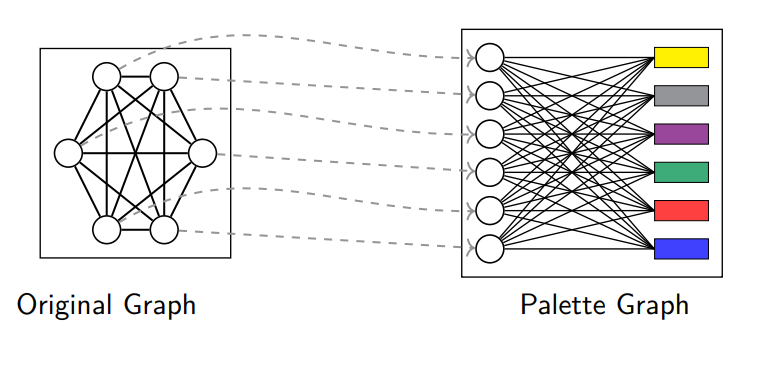
\includegraphics[width=0.5\textwidth]{images/Palette Graph 1.png}
		\end{center}
		
	\end{frame}
	
	\begin{frame}{Warm up: Special case}
		
		\begin{center}
			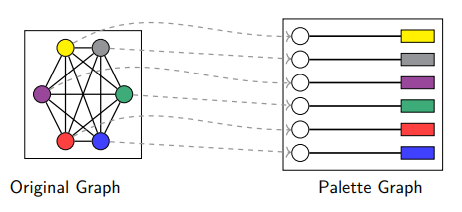
\includegraphics[width=0.5\textwidth]{images/Palette Graph 2.png}
		\end{center}
		
		\begin{itemize}
			\item The problem of finding a ($\Delta +1$) coloring in the original graph is equivalent to finding a perfect matching in the palette graph
		\end{itemize}
		
	\end{frame}
	
	\begin{frame}{Warm up: Special case}
		
		\begin{itemize}
			\item Relation with the Palette sparsification theorem: Random subgraphs of the palette graph of a clique contain a perfect matching
			(a result known from random graph theory)
		\end{itemize}
		\begin{center}
			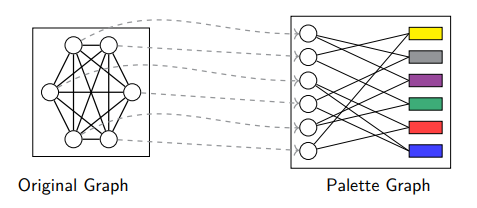
\includegraphics[width=0.5\textwidth]{images/Palette Graph 3.png}
		\end{center}
		
	\end{frame}
	
	\begin{frame}{Warm up: A more general case}
		
		\begin{itemize}
			\item Coloring a clique minus a perfect matching
			\item Suppose we have a clique and we remove a perfect matching from it
		\end{itemize}
		\begin{center}
			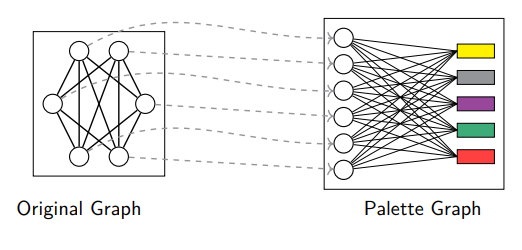
\includegraphics[width=0.5\textwidth]{images/Palette Graph 4.png}
		\end{center}
		\begin{itemize}
			\item ($\Delta +1$) coloring is equivalent to finding a \alert{good} subgraph in the palette graph
		\end{itemize}
		
	\end{frame}
	
	\begin{frame}{Warm up: A more general case}
		\begin{itemize}
			\item \alert{good}: When one color is assigned to more than one node, these nodes form an independent set in the original graph
		\end{itemize}
		\begin{center}
			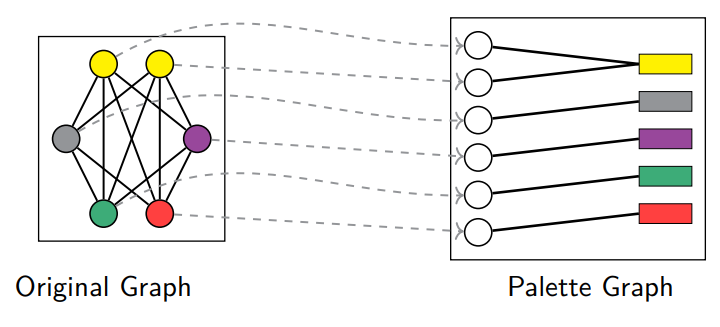
\includegraphics[width=0.5\textwidth]{images/Palette Graph 5.png}
		\end{center}
		\begin{itemize}
			\item Relation to the Palette sparsification theorem: Random subgraphs of the palette graph of a clique minus a perfect matching contain a good subgraph
		\end{itemize}
		
	\end{frame}
	
	\begin{frame}{A general method for almost cliques}
		\begin{itemize}
			\item When our graphs are close to being a clique:
			\newline
			\item Find a subgraph of the palette graph:
			\item Degree exactly one for vertices on left.
			\item Neighbors of vertices on right can only be an independent set in the original graph.
			\item Palette sparsification theorem reduces to a random graph theory question
			\newline
			\item \alert{ not that helpful for graphs that are far from cliques }
		\end{itemize}
		
	\end{frame}
	
	\begin{frame}{Graphs that are far from cliques}
		\begin{itemize}
			\item We will consider low degree graphs, like a  graph where all vertices have degree less than or equal to $ \Delta/2$
			\item (Every vertex except for one, has degree $<= \Delta/2$)
			
		\end{itemize}
		
	\end{frame}
	
	\begin{frame}{Low degree graphs}
		\begin{itemize}
			\item Our coloring strategy:
			\newline
			\begin{enumerate}
				\item Pick a color uniformly at random from $\{1, \ldots, \Delta + 1\}$ for all uncolored vertices.
				\item Assign the color to each vertex if it is not assigned to its neighbors in this iteration or previous ones.
				\item Repeat until all vertices are colored.
			\end{enumerate}
			\item Every vertex has constant probability of being colored in each iteration \\(In the worst case we have $\Delta$/2 neighbors of different colors, so this constant is at least 1/2)
			\item After O(log n) iterations, all vertices are colored
			
		\end{itemize}
		
	\end{frame}
	
	\begin{frame}{Why O(log n) iterations? }
		\begin{itemize}
			\item Let’s say at the start of an iteration, there are k uncolored vertices
			\item Each uncolored vertex gets colored independently with probability at least c (constant)
			\item So after one iteration, the expected number of uncolored vertices is at most $(1-c)*k$
			\item After t iterations, expected uncolored vertices $<= (1-c)^t*n$
			
		\end{itemize}
	\end{frame}
	
	\begin{frame}{Why O(log n) iterations? }
		\begin{itemize}
			\item We want this to be less than 1 to ensure all vertices are colored with high probability: \[ (1 - c)^t \cdot n < 1 \] Taking logarithms on both sides: \[ t \log(1 - c) + \log n < 0 \] \[ t > \frac{-\log n}{\log(1 - c)} \] Since \( c \) is a constant, \( \log(1 - c) \) is also constant (and negative), so \( \frac{-1}{\log(1 - c)} \) is a constant. Therefore: \[ t = O(\log n) \]
		\end{itemize}
	\end{frame}
	
	\begin{frame}{General proof}
		\begin{itemize}
			\item We have seen proofs for extreme cases, but what about the general case of a graph?
			\item Neither strategy works for the other case
			\item The strategy for coloring low degree graphs provably requires $\Omega(\Delta)$ iterations on a clique
			\item The strategy for coloring a clique is not appropriate for low-degree graphs since they lack structure
			
		\end{itemize}
		
	\end{frame}
	
	\begin{frame}{High Level Idea}
		\begin{itemize}
			\item We can decompose a given graph into \alert{dense} and \alert{sparse} sections
			
		\end{itemize}
		\begin{center}
			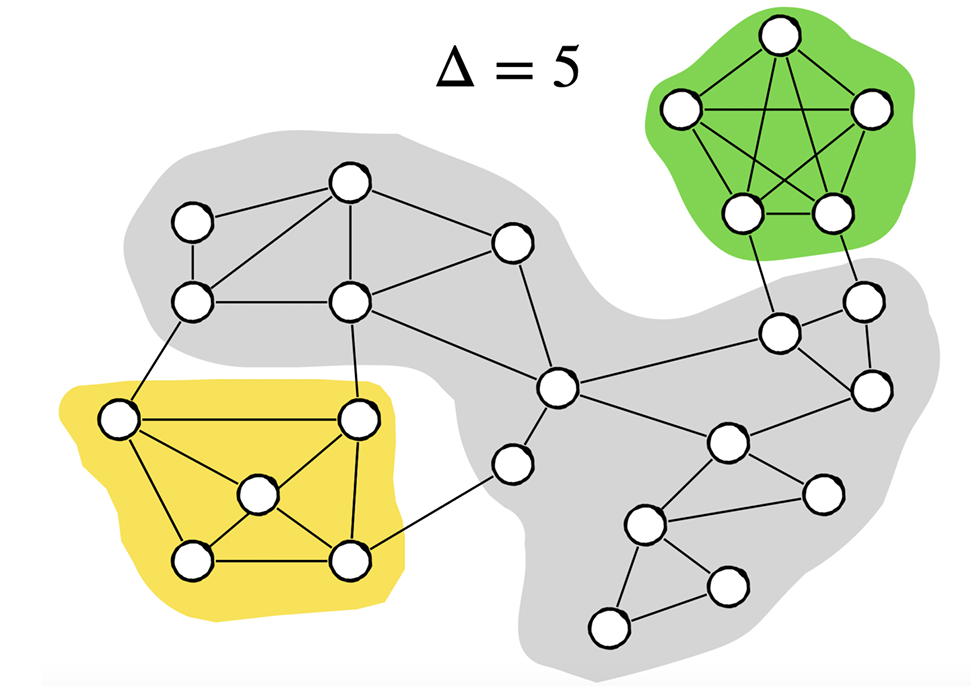
\includegraphics[width=0.5\textwidth]{images/Graph decomp.png}
		\end{center}
		
	\end{frame}
	
	\begin{frame}{Decomposition of A Graph}
		\begin{itemize}
			\item We use a simple extension of the decomposition of Harris, Schneider, and Su {\color{green!50!black}[Harris et al., 2016]} for distributed ($\Delta$ + 1) coloring
			\newline
			\item {\color{Blue}Extended HSS Decomposition}: For any $\epsilon \in$  (0, 1), any graph $G(V, E)$ can be decomposed into:
			\item \alert{Sparse vertices:} The neighborhood of each sparse vertex is missing at least $\varepsilon \cdot \binom{\Delta}{2}$ edges.
			
			\item \alert{A collection of almost-cliques:} Each almost-clique $C$:
			\begin{itemize}
				\item contains $(1 \pm \varepsilon)\Delta$ vertices.
				\item every vertex in $C$ has $\leq \varepsilon\Delta$ neighbors outside $C$.
				\item every vertex in $C$ has $\leq \varepsilon\Delta$ non-neighbors inside $C$.
			\end{itemize}
		\end{itemize}
		
	\end{frame}
	
	\begin{frame}{Sparse Vertices}
		\begin{itemize}
			\item A sparse vertex is a vertex who's neighborhood is $\epsilon$ far from being a clique
			\item If we look at the subgraph formed by all the neighbors of that vertex, it is missing $\epsilon$ fraction of edges of a clique
		\end{itemize}
		\begin{center}
			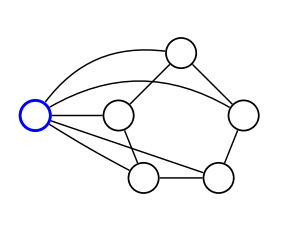
\includegraphics[width=0.2\textwidth]{images/sparse vertex.png}
		\end{center}
		\begin{itemize}
			\item With this description:
			\item Any low degree vertex is automatically a sparse vertex (Since we don't have enough edges to begin with)
			\item Some vertices that have a lot of edges connected to them may still be sparse (In the case where their neighborhood doesn't have any edges)
		\end{itemize}
	\end{frame}
	
	\begin{frame}{Almost Cliques}
		\begin{itemize}
			\item We can have multiple almost cliques
		\end{itemize}
		\begin{center}
			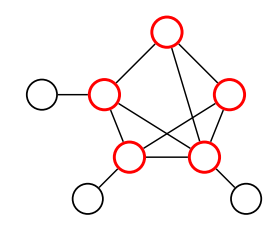
\includegraphics[width=0.3\textwidth]{images/Almost Clique.png}
		\end{center}
	\end{frame}
	
	\begin{frame}{Proof Strategy}
		\begin{enumerate}
			\item Fix an extended HSS decomposition of the graph for $\varepsilon \approx 0.001$
		\end{enumerate}
		\begin{center}
			\begin{minipage}{0.45\textwidth}
				\centering
				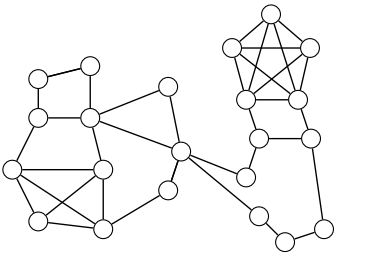
\includegraphics[width=\textwidth]{images/input graph.png}
			\end{minipage}
			\hfill
			\begin{minipage}{0.45\textwidth}
				\centering
				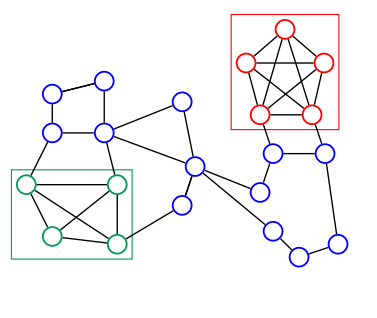
\includegraphics[width=\textwidth]{images/Decomposed graph.png}
			\end{minipage}
		\end{center}
	\end{frame}
	
	\begin{frame}{Proof Strategy}
		\begin{enumerate}
			\setcounter{enumi}{1}
			\item Use the first half of colors in $L(\cdot)$ to color sparse vertices
		\end{enumerate}
		\begin{center}
			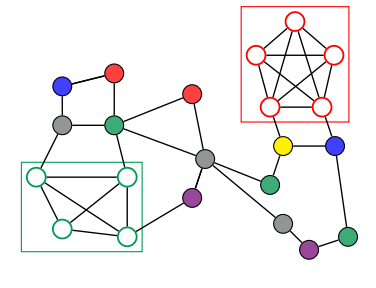
\includegraphics[width=0.5\textwidth]{images/half colored graph.png}
		\end{center}
	\end{frame}
	
	\begin{frame}{Proof Strategy}
		\begin{enumerate}
			\setcounter{enumi}{2}
			\item Iterate over the almost-cliques one by one and color each
			one using the remaining half of L(·)
		\end{enumerate}
		\begin{center}
			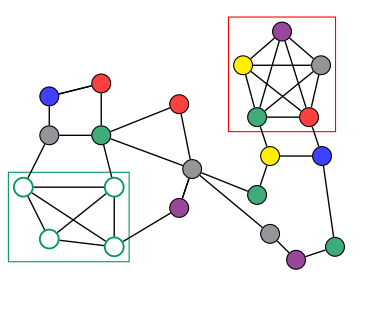
\includegraphics[width=0.5\textwidth]{images/more colored graph.png}
		\end{center}
	\end{frame}
	
	\begin{frame}{The main challenges}
		\begin{itemize}
			\item The size of the almost clique can be very large O($1+\epsilon\Delta$)
			\item The palette graph is not a complete bipartite graph since vertices in an almost-clique may have some colored neighbors outside
			
		\end{itemize}
		\begin{center}
			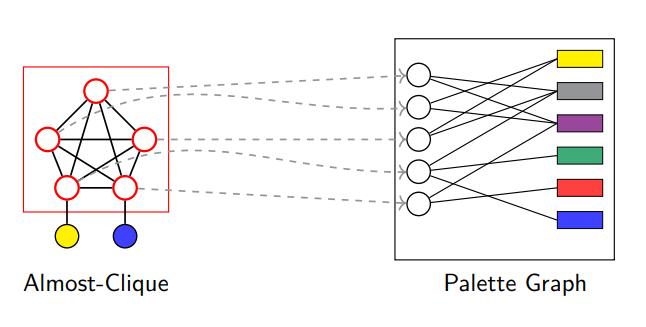
\includegraphics[width=0.5\textwidth]{images/challenge graph.png}
		\end{center}
	\end{frame}
	
	\section{Related Works}
	
	\begin{frame}
		\centering
		\Huge
		\textbf{Extensions of the Palette\\Sparsification Theorem}
	\end{frame}
	
	\begin{frame}{DISTRIBUTED $(\Delta + 1)$-COLORING IN SUBLOGARITHMIC ROUNDS}
		\begin{itemize}
			\item Goal: \textbf{$(\Delta + 1)$-coloring} in \textcolor{OrangeRed}{LOCAL} model.
			\item Runtime:
			\[
			\textcolor{ForestGreen}{O\left(\sqrt{\log \Delta}\right)} + \textcolor{ForestGreen}{2^{O\left(\sqrt{\log \log n}\right)}}
			\]
			
			\item \textbf{\textcolor{cyan}{Step 1: Classify Nodes}}
			\begin{itemize}
				\item \textcolor{YellowOrange}{Dense:} neighbors are mostly connected (almost clique).
				\item \textcolor{SkyBlue}{Sparse:} not dense.
				\item Done locally in \textcolor{green}{$O(1)$} rounds.
			\end{itemize}
			
			\item \textbf{\textcolor{cyan}{Step 2: Handle Dense Components}}
			\begin{itemize}
				\item Each dense part has weak diameter $\leq 2$.
				\item \textcolor{magenta}{Elect a leader} in 2 rounds to assign colors centrally.
				\item Most dense nodes are colored in one coordinated step.
			\end{itemize}
		\end{itemize}
	\end{frame}
	
	\begin{frame}{Shrinking, Finishing, and Final Runtime}
		\begin{itemize}
			\item \textbf{\textcolor{cyan}{Shrink Dense Parts}}:
			\begin{itemize}
				\item Each round reduces size by $1 - \Theta(\sqrt{\delta})$
				\item After $\left\lceil \sqrt{\log \Delta} \right\rceil$ rounds: $\tilde{O}(1)$-size
			\end{itemize}
			
			\item \textbf{\textcolor{cyan}{Sparse Remainder}}:
			\begin{itemize}
				\item Each sparse node has \textcolor{green}{$\Omega(\varepsilon^2 \Delta)$} colors and only \textcolor{red}{$O(\log n)$} live neighbors.
				\item Elkin–Pettie–Su list coloring in:
				\[
				\textcolor{ForestGreen}{O(\log(1/\varepsilon)) + 2^{O(\sqrt{\log \log n})}}
				\]
			\end{itemize}
			
			\item \textbf{\textcolor{cyan}{Tiny Residual Graph}}:
			\begin{itemize}
				\item Degree is \textcolor{orange}{$O(\log n) \cdot 2^{O(\sqrt{\log \Delta})}$}
				\item Final coloring using Barenboim–Elkin:
				\[
				\textcolor{ForestGreen}{O(\sqrt{\log \Delta}) + 2^{O(\sqrt{\log \log n})}}
				\]
			\end{itemize}
		\end{itemize}
	\end{frame}
	
	\begin{frame}{Palette Sparsification with Fewer Colors}
		\vspace{0.2cm}
		Could we establish \textcolor{blue}{palette sparsification theorem} by sampling only \textcolor{red}{$O(1)$} colors at each vertex?
		
		\vspace{0.5cm}
		\textcolor{orange}{\textbf{Claim:}} There exist graphs such that if each vertex samples \textcolor{red}{$o(\log n)$} colors, then almost certainly no feasible coloring exists among sampled colors.
		
		\vspace{0.5cm}
		\begin{itemize}
			\item Suppose $G$ consists of $n / \log n$ copies of the graph $K_{\log n}$.
			\item Then if each vertex samples \textcolor{red}{$o(\log n)$} colors, then almost certainly some clique fails to sample \textcolor{red}{$\log n$} distinct colors.
			\item So almost certainly no valid coloring exists among sampled colors.
		\end{itemize}
	\end{frame}
	
	\begin{frame}{Very Recent Work}
		\vspace{0.2cm}
		In fact, if we want a vanishingly small failure probability, we need to sample more than \textcolor{red}{\(\log n\)} colors at each vertex.
		
		\vspace{0.3cm}
		How big does the constant hidden in \textcolor{red}{\(O(\log n)\)} need to be?
		
		\vspace{0.6cm}
		\textbf{\textcolor{orange}{Asymptotically Optimal Version [Kahn and Kenney '23]}}
		
		\vspace{0.3cm}
		For any \(\varepsilon > 0\), if each vertex in a graph \(G\) independently samples \((1 + \varepsilon)\log n\) colors uniformly at random from \(\{1, 2, \ldots, \Delta + 1\}\), then w.h.p. there is a valid \textcolor{blue}{coloring} of the graph \(G\) such that each vertex is assigned one of its \textcolor{blue}{sampled colors}.
	\end{frame}
	
	\begin{frame}{(Degree + 1) Coloring}
		\vspace{0.2cm}
		The greedy coloring algorithm for \textcolor{red}{(\(\Delta+1\))}-coloring also works if we restrict each vertex \(v\) to only use colors from an \textcolor{blue}{arbitrary subset} of \textcolor{red}{(\(\deg(v) + 1\))} colors.
		
		\vspace{0.6cm}
		\textbf{(Degree + 1) Palette Sparsification}
		
		\vspace{0.2cm}
		\textbf{[Assadi and Alon '20]}\\
		\vspace{0.4cm}
		Palette sparsification theorem holds even if each  vertex \(v\) samples \textcolor{red}{\(O(\log n)\)} colors from \(\{1, 2, \ldots, \deg(v)+1\}\).
		
		\vspace{0.4cm}
		\textbf{[Halldorsson, Kuhn, Nolin, Tonoyan '22]}\\
		Extend it to \textcolor{blue}{arbitrary subsets} of \textcolor{red}{(degree + 1)} colors.
	\end{frame}
	
	\begin{frame}{\(\Delta\)-Coloring in Streams}
		
		\textbf{\textcolor{blue}{Brooks theorem}}: All graphs other than cliques and odd cycles are \(\Delta\)-colorable.
		
		\vspace{1em}
		
		\textbf{\textcolor{orange}{Streaming Brooks Theorem}} \textcolor{black}{[Assadi, Kumar, and Mittal '22]}\\
		There is a \(\tilde{O}(n)\) space single-pass streaming algorithm that can color any \(\Delta\)-colorable graph with \(\Delta\) colors.
		
	\end{frame}
	
	\begin{frame}{Palette Sparsification for \textit{C}-Coloring}
		
		\textbf{Does a similar sparsification result hold for \textcolor{red}{C}-colorable graphs for \textcolor{red}{C} $\leq \Delta$?}
		
		\vspace{1em}
		
		\textbf{\textcolor{orange}{Claim:}} There exist $\Delta$-colorable graphs such that unless each vertex samples $\Omega(\Delta^{0.5})$ colors, w.h.p. there is no feasible coloring exists among the sampled colors.
		
		\vspace{1em}
		
		\begin{itemize}
			\item Consider the graph $K_{\Delta+1}$ and remove an edge between any pair $u, v$ of vertices — this is a $\Delta$-colorable graph.
			\item In any $\Delta$-coloring, $u$ and $v$ must receive the same color.
			\item But unless each of $u$ and $v$ samples at least $\Omega(\Delta^{0.5})$ colors, it is unlikely they have a common color.
		\end{itemize}
		
	\end{frame}
	
	\begin{frame}{Other Extensions}
		
		Sublinear algorithms for coloring in terms of other natural parameters.
		
		\vspace{1em}
		
		A graph \textcolor{red}{$G$} has \textcolor{blue}{degeneracy} \textcolor{red}{$\kappa$} if every subgraph of \textcolor{red}{$G$} has a vertex of degree at most \textcolor{red}{$\kappa$}. The parameter \textcolor{red}{$\kappa$} is always at most \textcolor{red}{$\Delta$} but could be much smaller.
		
		\vspace{1em}
		
		\textcolor{orange}{[Bera, Chakrabarti, Ghosh’19]}
		\begin{itemize}
			\item Sublinear algorithms for coloring with \(\kappa + o(\kappa)\) colors.
			\item In contrast to \((\Delta+1)\)-coloring, the problem of finding a \((\kappa+1)\)-coloring turns out to be provably hard for both \textcolor{blue}{sublinear space} and \textcolor{blue}{time} algorithms.
		\end{itemize}
		
	\end{frame}
	
	\begin{frame}{Concluding Remarks}
		
		\begin{itemize}
			\item A \textcolor{blue}{non-adaptive sparsification} result for \textcolor{red}{(\(\Delta+1\))}-coloring.
			
			\vspace{0.5em}
			\item Any graph can be \textcolor{blue}{sparsified} to a graph with \(\tilde{O}(n)\) edges such that \textcolor{blue}{list-coloring} the sparsified graph is equivalent to \textcolor{red}{(\(\Delta+1\))}-coloring the original graph.
			
			\vspace{0.5em}
			\item The \textcolor{blue}{sparsification} yields \textcolor{blue}{essentially optimal} sublinear algorithms for three well-studied models of sublinear algorithms:
			\begin{itemize}
				\item \textcolor{red}{Streaming model} for \textcolor{blue}{sublinear space},
				\item \textcolor{red}{Query model} for \textcolor{blue}{sublinear time}, and
				\item \textcolor{red}{MPC model} for \textcolor{blue}{sublinear communication}.
			\end{itemize}
		\end{itemize}
		
	\end{frame}
	
	\begin{frame}{References}
		\footnotesize
		\bibliography{reference.bib}
		\bibliographystyle{apalike}
	\end{frame}
	
	\begin{frame}
		\Huge{\centerline{\textbf{Thank you!}}}
	\end{frame}
	
\end{document}
